\documentclass[oneside,11pt]{article}
\pdfoutput=1


%DONOTRUNBIBTEX


\usepackage{geometry}
\usepackage{amssymb,amsfonts}
\usepackage{mathtools}

\geometry{left=1.1in,right=1.1in,top=1.2in,bottom=1.2in}
\usepackage{natbib}
\bibliographystyle{plainnat}
\bibpunct{(}{)}{;}{a}{,}{,}
\usepackage[latin1]{inputenc}
\usepackage{mathrsfs}

\usepackage{color}
\usepackage[abs]{overpic}
\setlength\unitlength{1mm}
\usepackage{subfigure}
%\usepackage{algorithm}
\usepackage[ruled,vlined]{algorithm2e}

\usepackage[noend]{algpseudocode}
\usepackage{multirow}
\usepackage{amsmath, scalerel}

\usepackage{caption}
\usepackage{forloop}
\usepackage{hyperref}
\usepackage{amsthm}

\usepackage{xcolor}
\usepackage{framed}
\usepackage{lipsum}
\colorlet{shadecolor}{blue!20}

\usepackage{tablefootnote}
\hypersetup{
    colorlinks=true,
    linkcolor=magenta,
    filecolor=blue,      
    urlcolor=cyan,
}

\usepackage{url}
\usepackage{enumitem}
\setitemize{leftmargin=*}
\usepackage{amssymb}
\usepackage{amsmath}
\allowdisplaybreaks[3] 
\usepackage{bbold}
\usepackage{flafter}
\PassOptionsToPackage{pdftex}{graphicx}
\usepackage[pdftex]{graphicx}

\usepackage{fancyhdr}
 
\pagestyle{fancy}
\fancyhf{}
\fancyhead[LE,RO]{tliu@jacobs-alumni.de}
\fancyhead[RE,LO]{Tianlin Liu}
%\fancyfoot[CE,CO]{\leftmark}
\fancyfoot[LE,RO]{\thepage}
 

%%%%
%--------Theorem Environments--------
%theoremstyle{plain} --- default
\theoremstyle{definition}
\newtheorem{thm}{Theorem}[section]
\newtheorem{corr}[thm]{Corollary}
\newtheorem{prop}[thm]{Proposition}
\newtheorem{lemma}[thm]{Lemma}
\newtheorem{conj}[thm]{Conjecture}
\newtheorem{quest}[thm]{Question}
\newtheorem{defn}[thm]{Definition}
\newtheorem{defns}[thm]{Definitions}
\newtheorem{con}[thm]{Construction}
\newtheorem{exmp}[thm]{Example}
\newtheorem{exmps}[thm]{Examples}
\newtheorem{notn}[thm]{Notation}
\newtheorem{notns}[thm]{Notations}
\newtheorem{alg}[thm]{Algorithm}
\newtheorem{addm}[thm]{Addendum}
\newtheorem{exer}[thm]{Exercise}
\newtheorem{exerstar}[thm]{*Exercise}

%\theoremstyle{remark}
\newtheorem{rmk}[thm]{Remark}
\newtheorem{rems}[thm]{Remarks}
\newtheorem{warn}[thm]{Warning}

%%%%

\pdfinfo{
/Title (Notes on Markov Decision Process)
/Author (Tianlin Liu)}
%\setcounter{secnumdepth}{0}  



\newcommand{\dataset}{\mathcal{D}}
\newcommand{\RR}{\mathbb{R}}
\newcommand{\PP}{\mathbb{P}}
\newcommand{\EE}{\mathbb{E}}
\newcommand{\EEpi}{\mathbb{E}_{\pi}}
\newcommand{\Acal}{\mathcal{A}}
\newcommand{\Scal}{\mathcal{S}}
\newcommand{\Rcal}{\mathcal{R}}
\newcommand{\Tcal}{\mathcal{T}}

\newcommand{\vpi}{v_{\pi}}
\newcommand{\qpi}{q_{\pi}}
\newcommand{\qstar}{q_{\ast}}
\newcommand{\vstar}{v_{\ast}}
\newcommand{\Scalplus}{\mathcal{S}^{+}}
\newcommand{\N}{\mathbb{N}}
\newcommand{\indi}{\mathbb{1}}
\renewcommand\thesection{\arabic{section}}

\newcommand\givenbase[1][]{\:#1\lvert\:}
\let\given\givenbase
\newcommand\sgiven{\givenbase[\delimsize]}
\DeclarePairedDelimiterX\Basics[1](){\let\given\sgiven #1}



\DeclareMathOperator*{\argmin}{arg\,min}
\DeclareMathOperator*{\argmax}{arg\,max}
\DeclareMathOperator*{\bigcdot}{\scalerel*{\cdot}{\bigodot}}


  \SetKwInOut{Input}{inputs}
  \SetKwInOut{Output}{output}
  \SetKwProg{FindAnMFS}{FindAnMFS}{}{}
\SetKwFor{Loop}{RepeatForever}{}{EndLoop}

\newenvironment{solution}
{\renewcommand\qedsymbol{$\blacksquare$}\begin{proof}[Solution]} {\end{proof}}
  






\parindent0cm
\setlength{\parskip}{3mm}


\begin{document}

\title{Solutions to Exercises in Reinforcement Learning by Richard S. Sutton and Andrew G. Barto}
\vspace{2mm}


\author{ Tianlin Liu\\
Jacobs University Bremen\\
tliu@jacobs-alumni.de
}


\date{}

\maketitle

\tableofcontents

\section{The Reinforcement Learning Problem}

\begin{exer}
\emph{Self-Play}. Suppose, instead of playing against a random opponent, the reinforcement learning algorithm described above played against itself, with both sides learning. What do you think would happen in this case? Would it learn a different policy for selecting moves?
\end{exer}

\begin{shaded}
\begin{solution} 
 I would expect that after several games, both sides learn a set of moves, and it might be the case that they just keep playing that set of moves over and over. Since there is no new training data come in, the value function may stop updating.
 
 
\end{solution}
\end{shaded}

\begin{exer}
\emph{Symmetries}. Many tic-tac-toe positions appear different but are really the same because of symmetries. How might we amend the learning process described above to take advantage of this? In what ways would this change improve the learning process? Now think again. Suppose the opponent did not take advantage of symmetries. In that case, should we? Is it true, then, that symmetrically equivalent positions should necessarily have the same value?
\end{exer}

\begin{shaded}
\begin{solution} 

Exploiting symmetry can reduce the number of states we needed to characterize the game. In this case, we do not have to keep so many value numbers. I think we should take advantage of symmetries weather or not our opponent do. I would expect symmetrically equivalent positions have the same value, because the probability of winning/losing is the same for  symmetric states.




\end{solution}
\end{shaded}


\begin{exer}
\emph{Greedy Play.} Suppose the reinforcement learning player was greedy, that is, it always played the move that brought it to the position that it rated the best. Might it learn to play better, or worse, than a nongreedy player? What problems might occur?
\end{exer}

\begin{shaded}
\begin{solution} 
I would expect the the agent will learn to play worse than a non-greedy player. Suppose the agent always playing greedily, the agent chooses ``good'' moves according to its own experience. Since its experience might be partial or limited, the greedy choice might exclude some better moves, which could be selected if there are exploratory moves. 


\end{solution}
\end{shaded}



\begin{exer}
\emph{Learning from Exploration}. Suppose learning updates occurred after all moves, including exploratory moves. If the step-size parameter is appropriately reduced over time (but not the tendency to explore), then the state values would converge to a set of probabilities. What are the two sets of probabilities computed when we do, and when we do not, learn from exploratory moves? Assuming that we do continue to make exploratory moves, which set of probabilities might be better to learn? Which would result in more wins?
\end{exer}

\begin{shaded}
\begin{solution} 

The set of probabilities when we \emph{do not} learn from exploratory moves is the value we can achieve by performing (our assumed) optimal move. The set of probabilities when we \emph{do} learn from exploratory moves is the value we can achieve by performing (our assumed) optimal move corrupted by some random moves. I would expect the former is better and I will imagine it results more wins. We are interested to learn a policy which tells us what action to execute if a state is given. The exploratory move, however, is out of our interests: exploratory moves are just some random moves, which are not related to the state that the agent stands in.
\end{solution}
\end{shaded}



\begin{exer}
\emph{Other Improvements.} Can you think of other ways to improve the reinforcement learning player? Can you think of any better way to solve the tic-tac-toe problem as posed?
\end{exer}



\begin{shaded}
\begin{solution} 
For this 3-by-3 game, the state space is actually very small. It is possible to brute-force to specify the optimal moves for each and every board states.
\end{solution}
\end{shaded}



\section{Multi-arm Bandits}

\begin{exer}
In the comparison shown in Figure 2.2, which method will perform best in the long run in terms of cumulative reward and cumulative probability of selecting the best action? How much better will it be? Express your answer quantitatively.
\end{exer}

\begin{shaded}
\begin{solution} 
I would expect that the $\epsilon = 0.01$ method will perform best in the long run in terms of cumulative reward as well as cumulative probability of selecting the best action. 

In terms of cumulative reward: In the long run, the $\epsilon = 0.1$ method will achieve the reward of ($1.55 + \delta$), where $\delta$ is a noise with 0 mean and 1 variance, with probability of 0.9; the $\epsilon = 0.01$ method will achieve the reward of ($1.55 + \delta$), where $\delta$ is a noise with 0 mean and 1 variance, with probability of 0.99.  Hence $\epsilon = 0.1$ and $\epsilon = 0.01$ will achieve cumulative reward of $0.9 \times 1.55 = 1.395$ and $0.99 \times 1.55 = 1.5345$ respectively. 

In terms of cumulative probability of selecting the best action: In the long run, the $\epsilon = 0.1$ method will select the optimal action with probability 0.9; the $\epsilon = 0.01$ method will select the optimal action with probability 0.99. 


\end{solution}
\end{shaded}

\begin{exer}
If the step-size parameters, $\alpha_n$, are not constant, then the estimate $Q_n$ is a weighted average of previously received rewards with a weighting different from that given by (2.6). What is the weighting on each prior reward for the general case, analogous to (2.6), in terms of the sequence of step-size parameters?
\end{exer}


\begin{shaded}
\begin{solution} 


\begin{equation*} %\label{eq1}
\begin{split}
Q_{n+1} & \coloneqq Q_n + \alpha_n \left [ R_n - Q_n \right ] \\
& = Q_n + \alpha_n R_n. - \alpha_n Q_n \\
& = \alpha_n R_n + (1 - \alpha_n) \left [ \alpha_{n-1} R_{n-1} + (1 - \alpha_{n-1})Q_{n-1} \right ] \\
& = \Pi_{i =1}^{n} (1- \alpha_i)Q_1 + \sum_1^{n-1} \alpha_i \Pi_{j =i+1}^n (1- \alpha_j)R_i + \alpha_n R_n.
\end{split}
\end{equation*}



\end{solution}
\end{shaded}

\begin{exer}
(\textbf{programming}) Design and conduct an experiment to demonstrate the difficulties that sample-average methods have for nonstationary problems. Use a modified version of the 10-armed testbed in which all the $\qstar(a)$ start out equal and then take independent random walks. Prepare plots like Figure 2.2 for an action-value method using sample averages, incrementally computed by $\alpha = \frac{1}{n}$ , and another $n$ action-value method using a constant step-size parameter, $\alpha = 0.1$. Use $\epsilon = 0.1$ and, if necessary, runs longer than 1000 steps.
\end{exer}

\begin{shaded}
\begin{solution} 
Please see \texttt{exer2.3.py}.
\end{solution}
\end{shaded}



\begin{exer}
The results shown in Figure 2.3 should be quite reliable because they are averages over 2000 individual, randomly chosen 10-armed bandit tasks. Why, then, are there oscillations and spikes in the early part of the curve for the optimistic method? In other words, what might make this method perform particularly better or worse, on average, on particular early steps?
\end{exer}

\begin{shaded}
\begin{solution} 
The gap between different rewards is much larger in the early steps, which encourages the agent selects particular better or worse, on average, in early steps.

\end{solution}
\end{shaded}


\begin{exer}
In Figure 2.4 the UCB algorithm shows a distinct spike in performance on the 11th step. Why is this? Note that for your answer to be fully satisfactory it must explain both why the reward increases on the 11th step and why it decreases on the subsequent steps. Hint: if c = 1, then the spike is much less prominent.
\end{exer}

\begin{shaded}
\begin{solution}
\begin{itemize}
\item \textbf{The initial plateau:} This is due to the fact that actions are essentially selected randomly in early steps. Large c suppresses the action to select the action greedily. This makes the rewards low in early steps.

\item \textbf{The spike:} once a high-reward is reached by some almost randomly selected actions, the average reward for that step increases significantly.

\item \textbf{Decrease on subsequent move:} In the subsequent moves, C suppresses the agent keep selecting the high reward action, and therefore the reward is lowered. But because the Q for high-reward action has already been updated, there is still a reasonable chance to select that action. Hence the reward is not as low as before the spike.
 \end{itemize}
\end{solution}
\end{shaded}





\section{Finite Markov Decision Processes}

\begin{exer}
Devise three example tasks of your own that fit into the reinforcement learning framework, identifying for each its states, actions, and rewards. Make the three examples as different from each other as possible. The framework is abstract and flexible and can be applied in many different ways. Stretch its limits in some way in at least one of your examples.
\end{exer}

\begin{shaded}
\begin{solution} 
\begin{itemize}
\item  One the example is soccer-playing robots. Consider the simple case that a single robot is on the court. The states of the robot might be the grid position that it stands in. The action might be move north/south/west/east. The action might be (i) dribbling the ball and (ii) shooting the ball. The rewards might be 1 for each score and a small negative reward for each dribble-move. 

\item The second example is still the soccer playing robots. The action and rewards are the same as the previous example. What makes this example different is that, the states of the robot are not physical states, but a vector of probability distribution, which characterizes its prediction of possible future moves. This kind of states are used in OOM(Observable Operator Model) and PSR(Predictive State Representation) literatures.
 
\item The third example is solving Jigsaw puzzles. The states might be the arrangements of all pieces. The actions might be (i)exchange the position of two pieces and (ii) do nothing. Suppose if two pieces are put next to each other correctly, then they are locked together automatically by some oracle. The awards are (i) a small negative reward, say, 0.01, for each position exchange, (ii) a small positive reward, say, 0.1, for each ``lock'', and (iii) a large positive reward, say, 5, for completely solving the Jigsaw puzzles. 

\end{itemize}
\end{solution}
\end{shaded}


\begin{exer}
Is the reinforcement learning framework adequate to usefully represent all goal-directed learning tasks? Can you think of any clear exceptions?
\end{exer}

\begin{shaded}
\begin{solution}
One instance RI framework may fail is the case when \emph{reward hypothesis} (see section 3.2 of the book) is violated. Particularly, reward hypothesis fails to be true if we need a reward vector, instead of a reward scalar. Each entry of the reward vector might represent related but different goals that we might want to achieve. In this case, to maximize the reward, we have to do some trade-off between different goals, but the RL framework only considers a single goal.
\end{solution}
\end{shaded}



\begin{exer}
Consider the problem of driving. You could define the actions in terms of the accelerator, steering wheel, and brake, that is, where your body meets the machine. Or you could define them farther out?say, where the rubber meets the road, considering your actions to be tire torques. Or you could define them farther in?say, where your brain meets your body, the actions being muscle twitches to control your limbs. Or you could go to a really high level and say that your actions are your choices of where to drive. What is the right level, the right place to draw the line between agent and environment? On what basis is one location of the line to be preferred over another? Is there any fundamental reason for preferring one location over another, or is it a free choice?
\end{exer}


\begin{shaded}
\begin{solution}
I think the location depends on the goal of the given task. For instance, if the task aims to train human to make better  decision on braking or accelerating given the current traffic on the road, then the action at the level of ``brain meets body'' seems appropriate. If the task aims to train human to make better traveling plan, the actions at the level of ``choices of where to drive'' seems appropriate. If the tasks aims to assess and optimize the quality of the rubber, the actions where ``rubber meets the road'' seems appropriate.
\end{solution}
\end{shaded}



\begin{exer}
Suppose you treated pole-balancing as an episodic task but also used discounting, with all rewards zero except for $-1$ upon failure. What then would the return be at each time? How does this return differ from that in the discounted, continuing formulation of this task?
\end{exer}

\begin{shaded}
\begin{solution} 
The return will be $- \gamma^k$ as before, where $k$ is a time step in an episode. In the continuing formulation, it is helpful to have discounting factor: it prevents the return from blowing up to infinity. However, in episodic formulation, as we do not need to worry about infinite return, using discounting factor in this particular episodic setting seems meaningless: as our goal is to make the balance lasts as long as possible, we should make the reward of each additional time-step equally valuable, or even make each additional time-step that the balance lasts more valuable than its prior one, but certainly we do not want to discount the value of an additional time step-- it discourages the balance-time to last longer.
\end{solution}
\end{shaded}


\begin{exer}
Imagine that you are designing a robot to run a maze. You decide to give it a reward of +1 for escaping from the maze and a reward of zero at all other times. The task seems to break down naturally into episodes--the successive runs through the maze--so you decide to treat it as an episodic task, where the goal is to maximize expected total reward (3.1). After running the learning agent for a while, you find that it is showing no improvement in escaping from the maze. What is going wrong? Have you effectively communicated to the agent what you want it to achieve?
\end{exer}

\begin{shaded}
\begin{solution} 

The communication is not effective. We want to train the agent to escape from the maze as quick as possible, but the agent understand it in a way that, as long as it can escape from the maze, it does not matter how long it takes to escape. To effectively communicate what we want, we need to add a small negative reward for each step the agent moves. 
\end{solution}
\end{shaded}

\begin{exer}
\textbf{Broken Vision System}. Imagine that you are a vision system. When you are first turned on for the day, an image floods into your camera. You can see lots of things, but not all things. You can't see objects that are occluded, and of course you can't see objects that are behind you. After seeing that first scene, do you have access to the Markov state of the environment? Suppose your camera was broken that day and you received no images at all, all day. Would you have access to the Markov state then?
\end{exer}

\begin{shaded}
\begin{solution} 
After seeing that first scene, I do not have access to the Markov state of the environment. Markov state includes everything to predict the immediate future, but this certainly is not the case-- I can not see the objects behind me, and the object behind me, say, a car which about to run into the objects in front of me, may have an impact on the scene I would see in the immediate future.

Suppose my camera was broken for a whole day, certainly I do not have access to Markov state. The information I have is simply not enough to predict the future.
\end{solution}
\end{shaded}

\begin{exer}
What is the Bellman equation for action values, that is, for $q_{\pi}$? It must give the action value $q_{\pi}(s,a)$ in terms of the action values, $q_{\pi}(s',a')$, of possible successors to the state?action pair $(s,a)$. As a hint, the backup diagram corresponding to this equation is given in Figure 3.4 (right). Show the sequence of equations analogous to (3.12), but for action values.
\end{exer}

\begin{shaded}
\begin{solution} 
One direct corollary of Conditional Expectation Theorem is that, informally, we have 
\[ \EE [X \given \text{~info~}] = \sum_i \EE [X \given \text{~info},F_i] \PP(F_i \given \text{~info~}). \]
 \url{http://www.stat.yale.edu/~pollard/Courses/600.spring08/Handouts/elem.conditioning.pdf}

Before finding out what is $q_{\pi}(s',a')$, first we take a closer look at how $v_{\pi}(s)$ is deducted in the text. 

\begin{equation*} %\label{eq1}
\begin{split}
\vpi(s) & \coloneqq  \EE_{\pi}\left [G_t \given S_t = s \right ] \\
& = \EE_{\pi} \left [ \sum\limits_{k = 0}^{\infty} \gamma^k R_{t + k +1} \given S_t = s \right ]\\
& = \EE_{\pi} \left [ R_{t+1} + \gamma \sum\limits_{k = 0}^{\infty} \gamma^k R_{t + k +1} \given S_t = s \right ]\\
% & =  \sum\limits_{a} \pi(a\givens)  \sum\limits_{s',r} p(s', r \given s,a) \left [ r + \gamma \vpi(s') \right ], \forall s \in \Scal \\
& = \underbrace{\EE_{\pi} \left [ R_{t+1}\given S_t = s \right ]}_{\text{Part 1}} +  \underbrace{\EE_{\pi} \left [ \gamma \sum\limits_{k = 0}^{\infty} \gamma^k R_{t + k +1} \given S_t = s \right ]}_{\text{Part 2}}\\
\end{split}
\end{equation*}

\begin{equation*} %\label{eq1}
\begin{split}
\text{Part 1} & \coloneqq  \EE_{\pi} \left [ R_{t+1}\given S_t = s \right ] \\
& = \sum_a \EE_{\pi} \left [ R_{t+1}\given S_t = s, A_t = a \right ] \underbrace{\PP(a_t = a \given S_t = s)}_{\pi(a \given s)} \\
& = \sum_a \pi(a \given s) \sum_r r \PP(R_{t+1} = r \given S_t = s, A_t = a) \\
& = \sum_a \pi(a \given s) \sum_{s', r} r p(r,s' \given s,a) 
\end{split}
\end{equation*}


\begin{equation*} %\label{eq1}
\begin{split}
\text{Part 2} & \coloneqq  \EE_{\pi} \left [ \underbrace{\gamma \sum\limits_{k = 0}^{\infty} \gamma^k R_{t + k +1}}_{\coloneqq B} \given S_t = s \right ] \\
& = \sum_a \sum_{s'} \underbrace{\EE_{\pi} \left [ B \given S_t = s, A_t = a, S_{t+1} = s' \right ]}_{v_{\pi}(s')} \pi(a \given s) \PP(S_{t+1} = s' \given S_t = s, A_t = a) \\
& = \sum_a \pi(a \given s) \sum_{s',r} p(s', r \given s,a) v_{\pi}(s') \\
\end{split}
\end{equation*}

\[\text{Part 1} + \text{Part 2} =  \sum\limits_{a} \pi(a\given s)  \sum\limits_{s',r} p(s', r \given s,a) \left [ r + \gamma \vpi(s') \right ], \forall s \in \Scal \]

as desired.

Now, using the exactly the same idea
\begin{equation*} %\label{eq1}
\begin{split}
\qpi (s,a) & \coloneqq  \EE_{\pi}\left [G_t \given S_t = s, A_t = a \right ] \\
& = \EE_{\pi} \left [ \sum\limits_{k = 0}^{\infty} \gamma^k R_{t + k +1} \given S_t = s, A_t = a \right ]\\
& = \EE \left [ R_{t+1} + \gamma \sum_{k=0}^{\infty}\gamma^k R_{t+ k +2} | S_t = s, A_t = a \right ] \\
& = \underbrace{\EE \left [ R_{t+1}  | S_t = s, A_t = a \right ]}_{\text{Part 1}}+ \underbrace{\EE \left [\gamma \sum_{k=0}^{\infty}\gamma^k R_{t+ k +2} | S_t = s, A_t = a \right ]}_{\text{Part 2}} \\
\end{split}
\end{equation*}

\begin{equation*} %\label{eq1}
\begin{split}
\text{Part 1} & \coloneqq  \EE \left [ R_{t+1}  | S_t = s, A_t = a \right ] \\
& = \sum_{s',r} r p(s',r | s,a)
\end{split}
\end{equation*}

\begin{equation*} %\label{eq1}
\begin{split}
\text{Part 2} & \coloneqq  \EE \left [\underbrace{\gamma \sum_{k=0}^{\infty}\gamma^k R_{t+ k +2}}_{\coloneqq B} | S_t = s, A_t = a \right ] \\
 & = \sum_{s'} \EE \left [ B | S_t = s, A_t = a, S_{t+1} = s' \right ] \PP(S_{t+1} = s' \given S_t = s, A_t = a) \\
& = \sum_{s'} \sum_{a'} \underbrace{\EE \left [ B | S_t = s, A_t = a, S_{t+1} = s', A_{t+1} = a' \right ]}_{\gamma q_{\pi}(s',a')}~p(s' | s,a)~\underbrace{p(a' \given s')}_{\pi(a' \given s')} \\
& = \sum_{s'} p(s' | s,a) \sum_{a'} \gamma q_{\pi}(s',a')~\pi(a' \given s') \\
& = \sum_{s',r} p(s',r | s,a) \sum_{a'} \gamma q_{\pi}(s',a')~\pi(a' \given s')
\end{split}
\end{equation*}

\[ q_{\pi}(s,a) = \text{Part 1} + \text{Part 2} =  \sum\limits_{s', r} p(s',r \given s, a) \left [ r + \gamma \sum_{a'}  q_{\pi}(s', a') \pi(a' | s') \right ]\]

\end{solution}
\end{shaded}





\begin{exer}
The Bellman equation (3.12) must hold for each state for the value function $v_{\pi}$ shown in Figure 3.5 (right). As an example, show numerically that this equation holds for the center state, valued at +0.7, with respect to its four neighboring states, valued at +2.3, +0.4, -0.4, and +0.7. (These numbers are accurate only to one decimal place.)
\end{exer}

\begin{shaded}
\begin{solution} 

It is easy to read out the values in (3.12) from the Figure 3.5: $\pi(a|s) = 0.25$ for all $a$, $\gamma = 0.9$, $r= 0$, $p(s'| s, a) = 0.25$ for all a. Consequently,  

\[ 0.25\times 0.9 \times (2.3 + 0.4 - 0.4 + 0.7) \approx 0.7. \]
\end{solution}
\end{shaded}



\begin{exer}
In the gridworld example, rewards are positive for goals, negative for running into the edge of the world, and zero the rest of the time. Are the signs of these rewards important, or only the intervals between them? Prove, using (3.2), that adding a constant $c$ to all the rewards adds a constant, $v_c$, to the values of all states, and thus does not affect the relative values of any states under any policies. What is $v_c$ in terms of $c$ and $\gamma$?
\end{exer}


\begin{shaded}
\begin{solution} 
The signs matter in episodic tasks, as we will see in \textbf{exercise 3.10}. However, for continuing task, signs do not matter-- too see this, it is enough to prove the claim in this question.

Recall
\[ G_t  =  R_{t+1} + \gamma (R_{t+2} ) + \gamma^2 (R_{t+3} ) + \cdots \]
and
\[ V_{\pi}(s)  =  \EEpi [G_t | S_t = s]. \]

Let C be the constant we add for each reward,
\begin{equation*} %\label{eq1}
\begin{split}
\tilde{G_t} & =  R_{t+1} + \gamma (R_{t+2} +C) + \gamma^2 (R_{t+3} +C) + \cdots \\
 & = \sum_{k = 0}^{\infty} \gamma^k (R_{t+k+1}+ C) \\
 & = \underbrace{ \sum_{k = 0}^{\infty} \gamma^k R_{t+k+1}}_{G_t}+ \sum_{k = 0}^{\infty} \gamma^k C \\
\end{split}
\end{equation*}


and

\[ \tilde{V_{\pi}}(s)  =  \EEpi [G_t + \sum_{k = 0}^{\infty} \gamma^k C | S_t = s] = V_{\pi}(s) +  \sum_{k = 0}^{\infty} \gamma^k C = V_{\pi}(s) + \underbrace{\frac{C}{1 - \gamma}}_{ \coloneqq V_c}. \]

\end{solution}
\end{shaded}

\begin{exer}
Now consider adding a constant $c$ to all the rewards in an episodic task, such as maze running. Would this have any effect, or would it leave the task unchanged as in the continuing task above? Why or why not? Give an example.
\end{exer}
\begin{shaded}
\begin{solution} 
This will change the task. Consider the task of escaping from a maze. To accomplish the task, it is reasonable to assign a big positive reward, say, 10, for successfully escaping from the maze, and a small negative value, say, $-0.1$, for each step the agent moves. Adding a constant 1 to both 5 and -0.1, then there is a problem -- the agent will never escape from the maze, since it wants to stay as long as it can, to earn more positive reward by hovering around.
\end{solution}
\end{shaded}


\begin{exer}
The value of a state depends on the values of the actions possible in that state and on how likely each action is to be taken under the current policy. We can think of this in terms of a small backup diagram rooted at the state and considering each possible action.:

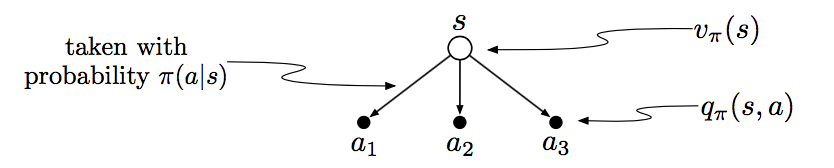
\includegraphics[width=14cm, height=3cm]{exer_3_11}

Give the equation corresponding to this intuition and diagram for the value at the root node, $v_{\pi}(s)$, in terms of the value at the expected leaf node, $q_{\pi}(s,a)$, given $S_t = s$. This equation should include an expectation conditioned on following the policy, $\pi$. Then give a second equation in which the expected value is written out explicitly in terms of $\pi(a|s)$ such that no expected value notation appears in the equation.
\end{exer}

\begin{shaded}
\begin{solution} 

First equation:

\begin{equation*} %\label{eq1}
\begin{split}
V_{\pi} & = \EEpi [G_t \given S_t = s] \\
 & =\sum_a \EEpi [G_t \given S_t = s, A_t = a] \PP[A_t = a \given S_t = s]. \\
\end{split}
\end{equation*}

Second equation follows from the first one:

\[ V_{\pi} = \sum_a q_{\pi}(s,a) \pi(a|s). \]




\end{solution}
\end{shaded}


\begin{exer}
The value of an action, $q_{\pi}(s,a)$, depends on the expected next reward and the expected sum of the remaining rewards. Again we can think of this in terms of a small backup diagram, this one rooted at an action (state?action pair) and branching to the possible next states:

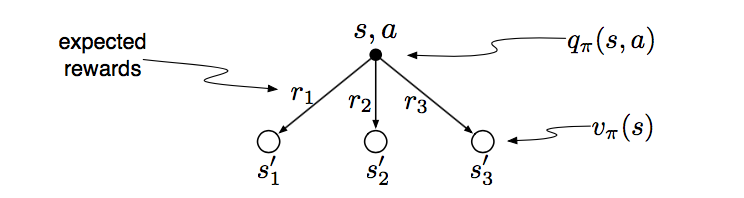
\includegraphics[width=13.5cm, height=3.3cm]{exer_3_12}

Give the equation corresponding to this intuition and diagram for the action value, $q_{\pi}(s,a)$, in terms of the expected next reward, $R_{t+1}$, and the expected next state value, $v_{\pi}(S_{t+1})$, given that $S_t = s$ and $A_t = a$. This equation should include an expectation but not one conditioned conditioned on following the policy. Then give a second equation, writing out the expected value explicitly in terms of $p(s',r|s,a)$ defined by (3.6), such that no expected value notation appears in the equation.
\end{exer}



\begin{shaded}
\begin{solution} 

First equation:

\begin{equation*} %\label{eq1}
\begin{split}
q_{\pi}(s,a) & = \EEpi [G_t \given S_t = s, A_t = a] \\
 & =\sum_{s'} \EEpi [G_t \given S_t = s, A_t = a, S_{t+1} = s'] \PP[S_{t+1} = s' \given S_t = s, A_t = a] \\
\end{split}
\end{equation*}

Second equation follows from the first one:

\begin{equation*} %\label{eq1}
\begin{split}
q_{\pi}(s,a) & =\sum_{s'} \EEpi [G_t \given S_{t+1} = s'] \PP[S_{t+1} = s' \given S_t = s, A_t = a] \\
& =  \sum_{s'} \EEpi [R_{t+1} + \gamma G_{t+1}  \given  S_t = s, A_t = a, S_{t+1} = s'] \PP[S_{t+1} = s' \given S_t = s, A_t = a] \\
& = \sum_{s',r} \left ( r + \gamma \underbrace{\EEpi [ G_{t+1}  \given  S_{t+1} = s']}_{\vpi(s')}  \right )p(s',r|s,a)\\
& = \sum_{s',r} \left [ r + \gamma \vpi(s')  \right ] p(s',r|s,a)\\
\end{split}
\end{equation*}




\end{solution}
\end{shaded}


\begin{exer}
Draw or describe the optimal state-value function for the golf example.
\end{exer}

\begin{shaded}
\begin{solution} 
I would expect the contour graph of optimal state-value function is looks similar as the lower figure of Figure 3.6, except the contour circle for -1 is larger-- it should covers the whole green. 

The reasoning is that, suppose we stand in anywhere outside of the green, then the optimal policy is to hit the ball into the green using driver, and then from the green we hit the ball into the hole using putter. Hence, if the location is outside of the green, the contour graph is exactly the same as $q_{\ast}(s, \text{driver})$. Now suppose we stand inside of green, unlike the case of $q_{\ast}(s, \text{driver})$, we do not commit ourself on first using the driver -- we are free to use putter in this case, and one stroke suffices to put the ball into the hole. Hence, inside of the green, the value is 1.
\end{solution}
\end{shaded}



\begin{exer}
Draw or describe the contours of the optimal action-value function for putting, $q_{\ast}(s,\text{putter})$, for the golf example.
\end{exer}

\begin{shaded}
\begin{solution} 
Suppose we stand in the green, and we commit ourself on first hitting the ball with a putter, then one stroke is enough -- value for the whole green is -1. Now suppose we stand outside of the green, and particular suppose we stand in the sand. Then committing ourself first hitting the ball with a putter, the first hit will result nothing, but subsequently we can use a driver and then another putter. So the value for the sand will be $-3$. Suppose we are further out, then the value will not be lower than that of $v_{\text{putter}}$. In this case, we commit to use the putter for the first hit, and then we can use as many as drivers as it is needed to reach the green, and another putter to put the ball into the hole.

\end{solution} 
\end{shaded}



\begin{exer}
Give the Bellman equation for $q_{\ast}$ for the recycling robot.
\end{exer}

\begin{shaded}
\begin{solution} 

\begin{equation*} %\label{eq1}
\begin{split}
\qstar(h,s) & = \underbrace{p(h \given h,s)}_{ \alpha} \left [ \underbrace{r(h,s,h)}_{r_{\text{search}}} + \gamma \max_{a'} \qstar(h,a')  \right ] + \underbrace{p(l \given h,s)}_{1- \alpha} \left[ \underbrace{r(h,s,l)}_{r_{\text{search}}} + \gamma \max_{a'} \qstar(l,a') \right ]\\
 & = r_{\text{search}} + \gamma \times \left [ \alpha \times \max_{a'} \qstar(h,a') + (1- \alpha) \times \max_{a'} \qstar(l,a')  \right ]. \\
\end{split}
\end{equation*}


% 2nd
\begin{equation*} %\label{eq1}
\begin{split}
\qstar(h,w) & = \underbrace{p(h \given h,w)}_{ 1} \left [ \underbrace{r(h,w,h)}_{r_{\text{wait}}} + \gamma \max_{a'} \qstar(h,a')  \right ] + \underbrace{p(l \given h, w)}_{0} \left[ \underbrace{r(h,w,l)}_{r_{\text{wait}}} + \gamma \max_{a'} \qstar(l,a') \right ]\\
 & = r_{\text{wait}} + \gamma \times \left [ \max_{a'} \qstar(h,a')  \right ]. \\
\end{split}
\end{equation*}

% 3rd
\begin{equation*} %\label{eq1}
\begin{split}
\qstar(l,s) & = \underbrace{p(h \given l,s)}_{1- \beta} \left [ \underbrace{r(l,s,h)}_{-3} + \gamma \max_{a'} \qstar(h,a')  \right ] + \underbrace{p(l \given l,s)}_{\beta} \left[ \underbrace{r(l,s,l)}_{r_{\text{search}}} + \gamma \max_{a'} \qstar(l,a') \right ]\\
 & = (1 - \beta) \left [ -3+  \gamma \max_{a'} \qstar(h,a') \right ] + \beta \left [ r_{\text{search}} + \gamma \max_{a'} \qstar(l,a') \right ]. \\
\end{split}
\end{equation*}

% 4th
\begin{equation*} %\label{eq1}
\begin{split}
\qstar(l,w) & = \underbrace{p(h \given l,w)}_{ 0} \left [ \underbrace{r(l,w,h)}_{r_{\text{wait}}} + \gamma \max_{a'} \qstar(h,a')  \right ] + \underbrace{p(l \given l, w)}_{1} \left[ \underbrace{r(l,w,l)}_{r_{\text{wait}}} + \gamma \max_{a'} \qstar(l,a') \right ]\\
 & = r_{\text{wait}} + \gamma \times \left [  \max_{a'} \qstar(l,a') \right ]. \\
\end{split}
\end{equation*}

% 5th
\begin{equation*} %\label{eq1}
\begin{split}
\qstar(l,r) & = \underbrace{p(h \given l,r)}_{ 1} \left [ \underbrace{r(l,r,h)}_{0} + \gamma \max_{a'} \qstar(h,a')  \right ] + \underbrace{p(l \given l,r)}_{0} \left[ \underbrace{r(l,r,l)}_{0} + \gamma \max_{a'} \qstar(l,a') \right ]\\
 & =  \gamma \times \left [  \max_{a'} \qstar(h,a') \right ]. \\
\end{split}
\end{equation*}
\end{solution} 
\end{shaded}




\begin{exer}
Figure 3.8 gives the optimal value of the best state of the gridworld as 24.4, to one decimal place. Use your knowledge of the optimal policy and (3.2) to express this value symbolically, and then to compute it to three decimal places.
\end{exer}

\begin{shaded}
\begin{solution} 

By definition,

\begin{equation*} %\label{eq1}
\begin{split}
\vstar(s) & = \max_{\pi} \vpi (s) \\
 & = \max_{\pi} \EE \left [G_t \given S_t = s \right ]. \\
\end{split}
\end{equation*}

It is easy to see that the optimal policy is do anything $\to$ go up $\to$ go up $\to$ go up $\to$ go up. Under this policy $\pi^\ast$, 

\begin{equation*} %\label{eq1}
\begin{split}
\vstar(s) & = \EE_{\pi^\ast} \left [ G_t \given S_t = s \right ] \\
& = \sum_{k = 0}^{\infty} \gamma^k \EE_{{\pi}^{\ast}} \left [ R_{t+k+1}  \given S_t = s \right ] \\
& = \sum_{j = 0}^{\infty} \gamma^{5j} \\
& = \frac{10}{1- \gamma^5} \\
& = \frac{10}{1- 0.9^5} \\
& \approx 24.419 \\
\end{split}
\end{equation*}


\end{solution} 
\end{shaded}

\section{Dynamic Programming}

\begin{exer}
In Example 4.1, if $\pi$ is the equiprobable random policy, what is $\qpi(11,\texttt{down})$? What is $\qpi$(7,\texttt{down})?
\end{exer}

\begin{shaded}
\begin{solution} 

Suppose we commit ourselves on going down from the position 11. Then we get a $-1$ reward deterministically, and the game is over (episode ends). Hence $\qpi(11,\texttt{down}) = -1$. 

Now suppose we commit ourselves on going down from position 7.  

\begin{equation*} %\label{eq1}
\begin{split}
\qpi(7,\texttt{down}) & = \EEpi [ G_t \given  S_t = s, A_t = a] \\
& = R_t + \underbrace{\gamma}_{1} \underbrace{\EE_\pi [ G_{t+1} \given S_{t+1} = s']}_{  v(11) } \\
& = -1 -14 \\
& = -15.
\end{split}
\end{equation*}


\end{solution} 
\end{shaded}

\begin{exer}
In Example 4.1, suppose a new state 15 is added to the gridworld just below state 13, and its actions, left, up, right, and down, take the agent to states 12, 13, 14, and 15, respectively. Assume that the transitions from the original states are unchanged. What, then, is $\vpi(15)$ for the equiprobable random policy? Now suppose the dynamics of state 13 are also changed, such that action down from state 13 takes the agent to the new state 15. What is $\vpi(15)$ for the equiprobable random policy in this case?
\end{exer}

\begin{shaded}
\begin{solution} 

Assume the transitions from the original states are unchanged. 

\begin{equation*} %\label{eq1}
\begin{split}
\vpi(15) & = \sum_a \underbrace{\pi(a|s)}_{0.25} \sum_{s', r} \underbrace{p(s' , r \given s,a)}_{1} [\underbrace{r}_{-1} + \underbrace{\gamma}_{1} \vpi(s')] \\
& =  0.25 (-1 - 22 - 1 - 20 - 1 -14 - 1 + \vpi(15))\\
\end{split}
\end{equation*}

Solve the above equation gives us $\vpi(15) = -20$.

Now suppose the dynamics of 13 also changed. We do the iterative policy evaluation. The initialization is natural: we let $V_0(s) = \vpi(s)$, where $\vpi$ is the value when the dynamics are unchanged, as shown in the $k = \infty$ case in Figure 4.1. Note that, especially, $V_0(15) = -20$, where $-20$ is what we just derived for $\vpi(15)$.

Particularly, we do the ``immediate overwriting''. First we update the value of 13. 

\begin{equation*} %\label{eq1}
\begin{split}
V_1(13) & = \sum_a \underbrace{\pi(a|s)}_{0.25} \sum_{s', r} \underbrace{p(s' , r \given s,a)}_{1} [\underbrace{r}_{-1} + \underbrace{\gamma}_{1} V_0(s')] \\
& =  0.25 (-1 - 20 - 1 - 22 - 1 -14 - 1 -20 )\\
& =  20 \\
\end{split}
\end{equation*}

Then we immediate update $V_1(15)$ using the updated $V_1(13)$. Note this is ``overwriting''.

\begin{equation*} %\label{eq1}
\begin{split}
V_1(15) & = \sum_a \underbrace{\pi(a|s)}_{0.25} \sum_{s', r} \underbrace{p(s' , r \given s,a)}_{1} [\underbrace{r}_{-1} + \underbrace{\gamma}_{1} V_0(s')] \\
& =  0.25 (-1 - 22 - 1 - 20 - 1 -14 - 1 - 20)\\
& =  20 \\
\end{split}
\end{equation*}

As we proceed, we will see nothing is changed -- the initialization is good enough. Hence the iterative policy evaluation ends with 1 iteration. $V_1(15)  = -20$ for this case.


\end{solution} 
\end{shaded}




\begin{exer}
What are the equations analogous to (4.3), (4.4), and (4.5) for the action-value function $\qpi$ and its successive approximation by a sequence of functions $q_0, q_1, q_2, \cdots$?
\end{exer}


\begin{shaded}
\begin{solution} 

Equations that are analogous to (4.3) and (4.4)
\begin{equation*} %\label{eq1}
\begin{split}
\qpi(s,a) & =\EEpi [G_t \given G_t = s, A_t = a] \\
& = \EEpi [R_{t+1} + \gamma V_{\pi}(S_{t+1}) \given S_t = s, A_t = a]\\
& = \EEpi [R_{t+1} + \gamma \sum_{a'} \pi(a'|s')\qpi(s',a') \given S_t = s, A_t = a ]\\
& = \sum\limits_{s', r} p(s',r \given s, a) \left [ r + \gamma \sum_{a'}  q_{\pi}(s', a') \pi(a' | s') \right ].
\end{split}
\end{equation*}

The equation that is analogous to (4.5)
\[ q_{k+1}(s,a) = \sum\limits_{s', r} p(s',r \given s, a) \left [ r + \gamma \sum_{a'}  q_{k}(s', a') \pi(a' | s') \right ]. \]


\end{solution} 
\end{shaded}


\begin{exer}
In some undiscounted episodic tasks there may be policies for which eventual termination is not guaranteed. For example, in the grid problem above it is possible to go back and forth between two states forever. In a task that is otherwise perfectly sensible, $\vpi(s)$ may be negative infinity for some policies and states, in which case the algorithm for iterative policy evaluation given in Figure 4.1 will not terminate. As a purely practical matter, how might we amend this algorithm to as- sure termination even in this case? Assume that eventual termination is guaranteed under the optimal policy.
\end{exer}


\begin{shaded}
\begin{solution} 

We can restricted to considering only policies that are $\epsilon$-soft, as shown in \textbf{exercise 4.7}. In this way, we will avoid trapping in some fixed loops, and every step our agent takes will have some chance to freely explore its world.  


\end{solution} 
\end{shaded}

\begin{exer}
 \textbf{(programming)} Write a program for policy iteration and re-solve Jack's car rental problem with the following changes. One of Jack's employees at the first location rides a bus home each night and lives near the second location. She is happy to shuttle one car to the second location for free. Each additional car still costs \$2, as do all cars moved in the other direction. In addition, Jack has limited parking space at each location. If more than 10 cars are kept overnight at a location (after any moving of cars), then an additional cost of \$4 must be incurred to use a second parking lot (independent of how many cars are kept there). These sorts of nonlinearities and arbitrary dynamics often occur in real problems and cannot easily be handled by optimization methods other than dynamic programming. To check your program, first replicate the results given for the original problem. If your computer is too slow for the full problem, cut all the numbers of cars in half.
\end{exer}

\begin{shaded}
\begin{solution} 


\end{solution} 
\end{shaded}


\begin{exer}
How would policy iteration be defined for action values? Give a complete algorithm for computing $\qstar$, analogous to that on page 87 for computing $\vstar$. Please pay special attention to this exercise, because the ideas involved will be used throughout the rest of the book.
\end{exer}


\begin{shaded}
\begin{solution} 
~\\

\begin{algorithm}[H]
 \caption{Policy iteration (using $q(s,a)$)}
 1. \Input{ $\qstar(s,a) = 0$, for all $s \in \Scalplus$ and $a \in \Acal$.\\}
  ~\\

2. \tcc{The policy evaluation step}
 \Repeat{ $\Delta < \theta$ (a small positive number) }{ 
  $\Delta \gets$ 0\;
  \ForEach{$(s,a) \in (\Scal \times \Acal )$}{
	$q \gets \qstar (s,a)$\;
        $\qstar (s,a) \gets \sum\limits_{s', r} p(s',r \given s, a) \left [ r + \gamma \sum_{a'}  q_{\pi}(s', a') \pi(a' | s') \right ]$ \;
        $\Delta \gets \max(\Delta, | q - \qstar(s,a)|)$
  }
 }
 ~\\
3.   \tcc{The policy improvement step}  
 policy-stable $\gets$ true. \\
 \ForEach{$s \in \Scal $}{
        old-action $\gets \pi(s)$ \;
        $\pi(s) \gets \argmax\limits_a \qstar(s,a)$ \;
        If old-action $\neq \pi(s)$, then policy-stale $\gets$ false.
  }
  If policy-stable, then stop and return $q \approx \qstar$ and $\pi \approx \pi_{\ast}$; else go to 2.
\end{algorithm}



\end{solution} 
\end{shaded}

\begin{exer}
Suppose you are restricted to considering only policies that are $\epsilon$-soft, meaning that the probability of selecting each action in each state, $s$, is at least $\epsilon/|A(s)|$. Describe qualitatively the changes that would be required in each of the steps 3, 2, and 1, in that order, of the policy iteration algorithm for $\vstar$ (page 87).
\end{exer}

\begin{shaded}
\begin{solution} 

For Step 3. Policy Improvement, instead of dictating the action specified by the argmax, we allow a uniform probability of $\frac{\epsilon}{|\Acal |- 1}$ for all other actions.


For Step 2 and 1, nothing need to be changed.

\end{solution} 
\end{shaded}



\begin{exer}
Why does the optimal policy for the gambler's problem have such a curious form? In particular, for capital of 50 it bets it all on one flip, but for capital of 51 it does not. Why is this a good policy?
\end{exer}

\begin{shaded}
\begin{solution} 


\end{solution} 
\end{shaded}


\begin{exer}
(\textbf{programming}) Implement value iteration for the gambler's problem and solve it for $p_h = 0.25$ and $p_h = 0.55$. In programming, you may find it convenient to introduce two dummy states corresponding to termination with capital of 0 and 100, giving them values of 0 and 1 respectively. Show your results graphically, as in Figure 4.3. Are your results stable as $\theta \to 0$?
\end{exer}

\begin{shaded}
\begin{solution} 


\end{solution} 
\end{shaded}


\begin{exer}
What is the analog of the value iteration backup (4.10) for action values, $q_{k+1}(s, a)$?
\end{exer}

\begin{shaded}
\begin{solution} 

We simply re-write (4.2) into an update equation.

\[ q_{k+1}(s,a) = \sum_{s',r} p(s',r | s,a ) \left [ r + \gamma \max_a q_{k}(s',a') \right ].  \]

\end{solution} 
\end{shaded}

\section{Monte Carlo Methods}

\begin{exer}
Consider the diagrams on the right in Figure 5.1. Why does the estimated value function jump up for the last two rows in the rear? Why does it drop off for the whole last row on the left? Why are the frontmost values higher in the upper diagrams than in the lower?
\end{exer}

\begin{shaded}
\begin{solution} 
%answer
(i) The estimated value function jump up for the last two rows in the rear because sticks at 21 and 20 has a high chance to win. (ii) It drops off for the whole last row on the left because if the dealer shows Ace, then the dealer has at least one Ace, which allows the dealer to have a reasonable chance to win or draw the game, compared to the case that the dealer has no Ace. (iii) The frontmost values higher in the upper diagrams than in the lower, because the Ace gives the flexibility of using it as 1 or 11, which is an advantage. Consider the case that the player sum is 12. If there is no usable Ace, and if the player gets an additional face card, the player goes bust. But suppose the player has a usable Ace, an additional face card is OK. The usable Ace provides the advantage for upper diagram.
\end{solution} 
\end{shaded}




\begin{exer}
What is the backup diagram for Monte Carlo estimation of $q_{\pi}$?
\end{exer}

\begin{shaded}
\begin{solution} 
%answer
I would expect the backup diagram looks like: filled circle (action) $\to$ circle (state)  $\to$  filled circle (action) $\to$ circle (state) $\cdots$ terminal state. \\

In fact, the diagram is given in Figure 7.3 of this book... It is the second diagram on the right: $\infty-$ step Sarsa aka Monte Carlo.

\end{solution} 
\end{shaded}






\begin{exer}
What is the equation analogous to (5.5) for action values $Q(s,a)$ instead of state values $V(s)$, again given returns generated using $\mu$?
\end{exer}

\begin{shaded}
\begin{solution} 
%answer
Similar to the case of V(s), we write
\[Q(s,a) = \frac{\sum_{t \in \mathcal{T}} \rho_t^{T(t)}G_t}{|\mathcal{T}(s,a)|}. \] 

In the above equation, for the every-visit method, $\Tcal(s,a)$ denotes the set of all time steps that $a$ is performed upon $s$; for the first-visit method, $\Tcal(s,a)$ denotes the first time that $a$ is performed upon $s$ in the episode. $ \{ G_t \}_{t \in \Tcal(s,a)}$ are the returns that pertain to the state-action pair $(s,a)$. $\{ \rho_t^{T(t)} \}_{t \in \Tcal(s)}$ are the importance -sampling ratio, which is defined as 

\[\rho_t^T = \frac{p(S_{t+1}|S_t, A_t) \prod_{k=t+1}^{T-1} \pi(A_k|S_k)p(S_{k+1} | S_k. A_k)}{p(S_{t+1}|S_t, A_t) \prod_{k=t+1}^{T-1} \mu(A_k|S_k)p(S_{k+1} | S_k. A_k)} =  \frac{ \prod_{k=t+1}^{T-1} \pi(A_k|S_k)}{ \prod_{k=t+1}^{T-1} \mu(A_k|S_k)} \]

\end{solution} 
\end{shaded}



\begin{exer}
In learning curves such as those shown in Figure 5.4 error generally decreases with training, as indeed happened for the ordinary importance-sampling method. But for the weighted importance-sampling method error first increased and then decreased. Why do you think this happened?
\end{exer}


\begin{shaded}
\begin{solution} 
%answer
This happens because weighted importance sampling is biased, though this bias converge to 0 asymptotically. 

\end{solution} 
\end{shaded}



\begin{exer}
The results with Example 5.5 and shown in Figure 5.5 used a first- visit MC method. Suppose that instead an every-visit MC method was used on the same problem. Would the variance of the estimator still be infinite? Why or why not?
\end{exer}

\begin{shaded}
\begin{solution} 
%answer
Following the argument in the textbook about the relationship between expectation and variance, we only need to show the expected square of the importance-sampling-scaled return is infinite. That is to say, we need to show:

\[ \EE \left [ \frac{\sum_{t \in \Tcal(s)} \rho_t^{T(t)}G_t}{ |\Tcal(s)|} \right ] = \infty \]

where $\Tcal(s)$ is the index set of all time steps in which state $s$ is visited.

Note that the equation used in the textbook for first-visit-MC method is a special case of the above equation: It makes $\Tcal = \{0\}$ and $|\Tcal| = 1$, i.e., it is just the first visit to $s$ within the episode. That is to say, in the textbook, we have shown

\[  \EE \left [ (\rho_0 G_0)^2 \right ] = \infty.  \]

But since returns are non-negative in this example,

 \[ \EE \left [ \frac{\sum_{t \in \Tcal(s)} \rho_t^{T(t)}G_t}{ |\Tcal(s)|} \right ] = \frac{1}{ |\Tcal(s)|} \EE \left [ \sum_{t \in \Tcal(s)} \rho_t^{T(t)}G_t \right ] \geq \frac{1}{ |\Tcal(s)|} \EE \left [ (\rho_0 G_0)^2 \right ] = \infty. \]

\end{solution} 
\end{shaded}



\begin{exer}
Modify the algorithm for first-visit MC policy evaluation (Section 5.1) to use the incremental implementation for sample averages described in Section 2.3.
\end{exer}

\begin{shaded}
\begin{solution} 
%answer
~\\
\begin{algorithm*}[H]
 \caption{First-visit MC Policy Evaluation (using incremental implementation) }
  \Input{  $\pi \gets$ policy to be evaluated \\
  $V(s) \gets 0$ for all $s$.\\
  $N(s) \gets 0$ for all $s$.\\ 
   Return($s$) $\gets$ an empty list, for all $s \in \Scal$\\

  }
 \Loop{}{ 
  Generate an episode using $\pi$\;
  \ForEach{ state $s$ appearing in the episode}{
	$G \gets $ return following the first occurence of s \;
	$N(s) \gets N(s) + 1$ \;
        $V(s) \gets V(s) + \frac{1}{N(s)} [G - V(s)]$ \;
  }
 }
\end{algorithm*}



\end{solution} 
\end{shaded}



\begin{exer}
Derive the weighted-average update rule (5.7) from (5.6). Follow the pattern of the derivation of the unweighted rule (2.3).
\end{exer}

\begin{shaded}
\begin{solution} 
%answer

\begin{equation*} %\label{eq1}
\begin{split}
V_{n+1} & = \frac{\sum_{k=1}^n W_k G_k}{ \sum_{k=1}^n W_k}\\
& = \frac{1}{ \sum_{k=1}^n W_k} \left [ W_n G_n + \sum_{k=1}^{n-1} W_k G_k \right ] \\
& = \frac{1}{ \sum_{k=1}^n W_k} \left [ W_n G_n + \left [  \sum_{k=1}^{n-1} W_k \right ] \underbrace{\frac{\sum_{k=1}^{n-1} W_k G_k}{ \sum_{k=1}^{n-1} W_k}}_{V_n} \right ] \\
& = V_n (1 - \frac{W_n}{\sum_{k=1}^n W_k}) + \frac{W_n G_n}{\sum_{k=1}^n W_k} \\
& = V_n + \frac{W_n}{C_n}\left [G_n - V_n \right ] \\
\end{split}
\end{equation*}
where $C_n = \sum_{k=1}^n W_k $.

\end{solution} 
\end{shaded}



\begin{exer}

\textbf{Racetrack (programming)}. Consider driving a race car around a turn like those shown in Figure 5.6. You want to go as fast as possible, but not so fast as to run off the track. In our simplified racetrack, the car is at one of a discrete set of grid positions, the cells in the diagram. The velocity is also discrete, a number of grid cells moved horizontally and vertically per time step. The actions are increments to the velocity components. Each may be changed by +1, -1, or 0 in one step, for a total of nine actions. Both velocity components are restricted to be nonnegative and less than 5, and they cannot both be zero except at the starting line. Each episode begins in one of the randomly selected start states with both velocity components zero and ends when the car crosses the finish line. The rewards are -1 for each step until the car crosses the finish line. If the car hits the track boundary, it is moved back to a random position on the starting line, both velocity components are reduced to zero, and the episode continues. Before updating the car?s location at each time step, check to see if the projected path of the car intersects the track boundary. If it intersects the finish line, the episode ends; if it intersects anywhere else, the car is considered to have hit the track boundary and is sent back to the starting line. To make the task more challenging, with probability 0.1 at each time step the velocity increments are both zero, independently of the intended increments. Apply a Monte Carlo control method to this task to compute the optimal policy from each starting state. Exhibit several trajectories following the optimal policy (but turn the noise off for these trajectories).


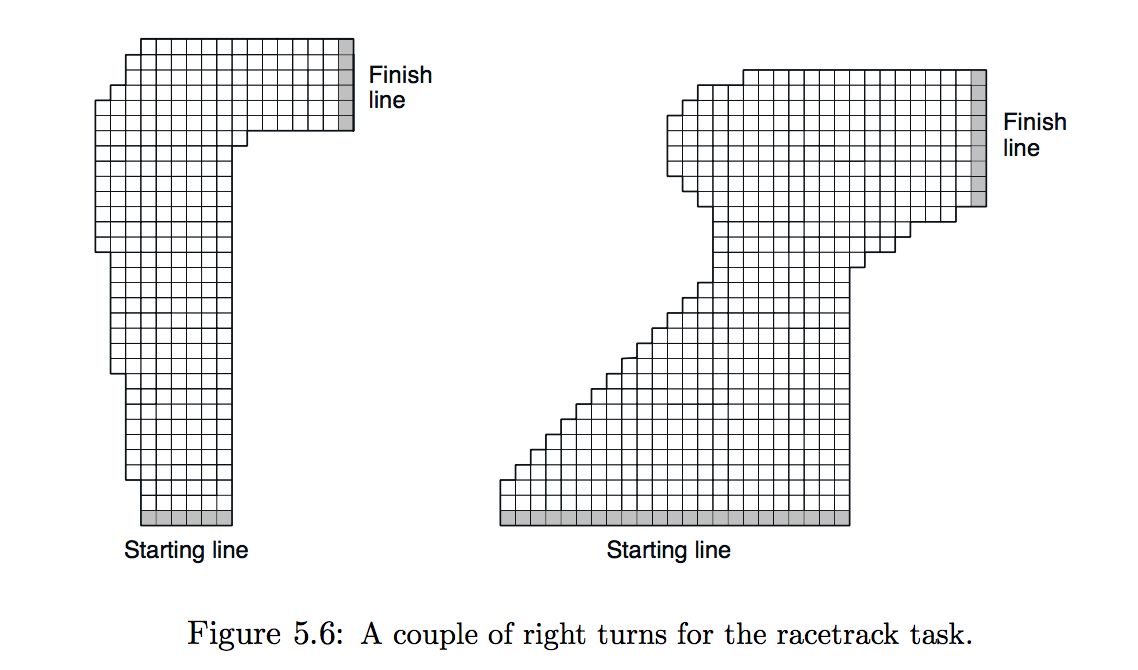
\includegraphics[width=14cm, height=8cm]{exer_5_8}


\end{exer}


\begin{shaded}
\begin{solution} 
%answer


\end{solution} 
\end{shaded}


\begin{exerstar}
Modify the algorithm for off-policy Monte Carlo control (page 119) to use the idea of the truncated weighted-average estimator (5.9). Note that you will first need to convert this equation to action values.
\end{exerstar}


\begin{shaded}
\begin{solution} 
%answer


\end{solution} 
\end{shaded}


\section{Temporal-Difference Learning}

\begin{exer}
This is an exercise to help develop your intuition about why TD methods are often more efficient than Monte Carlo methods. Consider the driving home example and how it is addressed by TD and Monte Carlo methods. Can you imagine a scenario in which a TD update would be better on average than a Monte Carlo update? Give an example scenario?a description of past experience and a current state?in which you would expect the TD update to be better. Here's a hint: Suppose you have lots of experience driving home from work. Then you move to a new building and a new parking lot (but you still enter the highway at the same place). Now you are starting to learn predictions for the new building. Can you see why TD updates are likely to be much better, at least initially, in this case? Might the same sort of thing happen in the original task?
\end{exer}

\begin{shaded}
\begin{solution} 
%answer
As long as I enter the highway, my estimates for the remaining time are supposed to be very accurate as a result of previous experience of driving home from work. In this case, it is reasonable to update my estimation for the remaining time once I enter the highway (which is the TD method), instead of only updating it once I arrive at home (which is the MC method). For this reason, TD updates are likely to be much better, at least initially. I assume the same sort of thing would happen in the original task, given that one can elaborate a prior knowledge of some relatively accurate estimations.

\end{solution} 
\end{shaded}


\begin{exer}
From Figure 6.2 (left) it appears that the first episode results in a change in only $V(A)$. What does this tell you about what happened on the first episode? Why was only the estimate for this one state changed? By exactly how much was it changed?
\end{exer}

\begin{shaded}
\begin{solution} 
%answer
~\\
(i)This tells me in the first episode, the random walk ended up in the right. \\
(ii) Suppose the random walk ends up in the right, one can see that only the estimate for A is changed-- suppose s' is not A, s is the previous state of s, then we have 

\[V(s) = \underbrace{V(s)}_{0.5} + \alpha \left [ \underbrace{R}_{0} + \underbrace{V(s')}_{0.5} - \underbrace{V(s)}_{0.5} \right ] = 0.5\]

(iii) Suppose the random walk ends up in the right, one can see that V(A) = 0.45

\[V(A) = \underbrace{V(A)}_{0.5} + \underbrace{\alpha}_{0.1} \left [ \underbrace{R}_{0} + \underbrace{V(\text{LeftBox})}_{0} - \underbrace{V(A)}_{0.5} \right ] = 0.45. \]
\end{solution} 
\end{shaded}

\begin{exer}
The specific results shown in Figure 6.2 (right) are dependent on the value of the step-size parameter, $\alpha$. Do you think the conclusions about which algorithm is better would be affected if a wider range of $\alpha$ values were used? Is there a different, fixed value of $\alpha$ at which either algorithm would have performed significantly better than shown? Why or why not?
\end{exer}

\begin{shaded}
\begin{solution} 
%answer


\end{solution} 
\end{shaded}


\begin{exerstar}
 In Figure 6.2 (right) the RMS error of the TD method seems to go down and then up again, particularly at high $\alpha$'s. What could have caused this? Do you think this always occurs, or might it be a function of how the approximate value function was initialized?
\end{exerstar}

\begin{shaded}
\begin{solution} 
%answer


\end{solution} 
\end{shaded}

\begin{exer}
6.5 Above we stated that the true values for the random walk task are $\frac{1}{6}, \frac{2}{6}, \frac{3}{6}, \frac{4}{6}$, and $\frac{5}{6}$, for states $A$ through $E$. Describe at least two different ways that these could have been computed. Which would you guess we actually used? Why?
\end{exer}

\begin{shaded}
\begin{solution} 
%answer
~\\
\begin{itemize}
\item \textbf{Method 1}: The true value of each state is the probability of terminating on the right if starting from that state. It is obvious that $x_C = 0.5$, as ending up in the left or right has the same probability for simple random walk. \\

Now Imagine if one stands in $D$, then one will go to C or go to E with equal probability. Once arrive at C, the probability of ending up in the right is given by $x_C$; once arrive at E, the probability of ending up in the right is given by $x_E$. Hence 

\[x_D = \PP(\text{go to C from D}) \times x_C + \PP(\text{go to E from E}) \times  x_E = \frac{x_C + x_E}{2}.\]

In the same fashion, one get 

\[x_A = \frac{x_{\text{LeftBox}} + x_B}{2}. \]
\[x_B = \frac{x_{A} + x_C}{2}. \]
\[x_E = \frac{x_{\text{RightBox}} + x_D}{2}. \]

Note $x_{\text{LeftBox}} = 0$, $x_{\text{LeftBox}} = 1$. Solving the above linear equations gives the desired results.
\item \textbf{Method 2} Use iterative value iteration bruteforcely. Since iterative value iteration guarantees to converge, the algorithm gives out desired values.
\end{itemize}

Method 1 is much easier, and therefore I assume the authors use the first one.

\end{solution} 
\end{shaded}

\begin{exerstar}
Design an off-policy version of the TD(0) update that can be used
with arbitrary target policy $\pi$ and covering behavior policy $\mu$, using at each step $t$ the importance sampling ratio $\rho_t^{t+1}$ (5.3).
\end{exerstar}

\begin{shaded}
\begin{solution} 
%answer


\end{solution} 
\end{shaded}


\begin{exer}
Re-solve the windy gridworld task assuming eight possible actions, including the diagonal moves, rather than the usual four. How much better can you do with the extra actions? Can you do even better by including a ninth action that causes no movement at all other than that caused by the wind?
\end{exer}

\begin{shaded}
\begin{solution} 
%answer


\end{solution} 
\end{shaded}


\begin{exer}
Re-solve the windy gridworld task with King's moves, assuming that the effect of the wind, if there is any, is stochastic, sometimes varying by 1 from the mean values given for each column. That is, a third of the time you move exactly according to these values, as in the previous exercise, but also a third of the time you move one cell above that, and another third of the time you move one cell below that. For example, if you are one cell to the right of the goal and you move \texttt{left}, then one-third of the time you move one cell above the goal, one-third of the time you move two cells above the goal, and one-third of the time you move to the goal.
\end{exer}

\begin{shaded}
\begin{solution} 
%answer


\end{solution} 
\end{shaded}


\begin{exer}
Why is Q-learning considered an off-policy control method?
\end{exer}

\begin{shaded}
\begin{solution} 
%answer
This is because, as has already been stated in the textbook, ``the learned action-value function, $Q$, directly approximates $Q^{\ast}$, the optimal action-value function, independent of the policy being followed.'' 

More specifically, to update $Q$ in each iteration in $Q$-learning, given $S$, $A$, $R$, and $S'$, we \emph{pretend} that we execute $a' = \argmax_a Q(S', a)$ for the next iteration. In other words, we pretend we execute the absolutely greedy action. It is a \emph{pretend}, as in the next iteration, we actually execute the $\epsilon-$greedy action. In this sense, we improve a policy which is different from that used to generate the data. Hence it is a off-policy method.

This solution partially owe to \url{https://stats.stackexchange.com/questions/184657/difference-between-off-policy-and-on-policy-learning}

\end{solution} 
\end{shaded}


\begin{exerstar}
What are the update equations for Double Expected Sarsa with an $\epsilon$-greedy target policy?
\end{exerstar}

\begin{shaded}
\begin{solution} 
%answer


\end{solution} 
\end{shaded}


\begin{exer}
Describe how the task of Jack's Car Rental (Example 4.2) could be reformulated in terms of afterstates. Why, in terms of this specific task, would such a reformulation be likely to speed convergence?
\end{exer}

\begin{shaded}
\begin{solution} 
%answer
The current definition of state in Jack's Car Rental problem is a tuple, in which each entry indicates the number of cars in a location at the end of the day. 

We can define the afterstates as a tuple, in which each entry is the number of cars in a location \emph{at the beginning of a day}. That is to say, the states are defined after the action, i.e., car-moving during the night, are executed.

This reformulation is likely to speed convergence, as this reformulation reduces the dimension of states. Consider the case (i) at the end of a day, Jack has 4 cars in location A and 8 cars in location B, and he decides to transport 2 cars from B to A; case (ii) In the end of a day, Jack has 6 cars in location A and 6 cars in location B, and he decides to do nothing. The cases (i) and (ii) boils down to the same aftertstate, namely, (6, 6).

\end{solution} 
\end{shaded}


\section{Multi-step Bootstrapping}

\begin{exer}
Why do you think a larger random walk task (19 states instead of 5) was used in the examples of this chapter? Would a smaller walk have shifted the advantage to a different value of $n$? How about the change in left-side outcome from 0 to 1 made in the larger walk? Do you think that made any difference in the best value of $n$?
\end{exer}


\begin{shaded}
\begin{solution}
~\\
\begin{itemize} 
 \item I would expect 5 states are too few to test the n-step TD if $n$ is fairly large, say, 64, 128, 256, 512 as shown in this example. It is very likely that the random walk reaches the terminal state using less than $n$ steps. Recall that the value function of n-step TD is not updated for the first $n-1$ step. Hence if the state number is significantly smaller than that of the $n$, it is very likely that $n$-step TD algorithm do nothing before it reaches the terminal states, and in this case, it is exactly the same as MC method. We want to test n-step TD method but not MC method.
 
 \item Following the same reasoning above, I would expect a smaller walk shifts to a different value of n. 

 \item I do not think changing in left-side outcome from 0 to 1 make any difference in the best value of $n$. But perhaps this speeds up the learning efficiency for n-step TD. As now the reward for achieving the left terminal state (= $-1$) is different from the reward for achieving any intermediate state ($= 0$), this difference makes the agent discern that, after $n$ steps, if it reaches the left terminal state or somewhere in the intermediate step.
 
 \end{itemize}

\end{solution} 
\end{shaded}

\section{Planning and Learning with Tabular Methods}


\begin{exer}
The nonplanning method looks particularly poor in Figure 8.4 because it is a one-step method; a method using multi-step bootstrapping would do better. Do you think one of the multi-step bootstrapping methods from Chapter 7 could do as well as the Dyna method? Explain why or why not.
\end{exer}


\begin{shaded}
\begin{solution} 
To my understanding, Dyna has two advantages: (i) it updates a set of values in an episode, instead of just one value as in the without-planning case (ii) it exploits the both ``learning from real experience'' and ``learning from simulated experience''. Now suppose we use a multi-step bootstrapping methods from Chapter 7, the advantage (i) vanishes as both methods enjoy this property, but the advantage (ii) of Dyna is not exploited by any multi-step bootstrapping method. For this reason, I would not expect one of the multi-step bootstrapping methods from Chapter 7 could do as well as the Dyna method. 

\end{solution} 
\end{shaded}


\begin{exer}
Why did the Dyna agent with exploration bonus, Dyna-Q+, perform better in the first phase as well as in the second phase of the blocking and shortcut experiments?
\end{exer}


\begin{shaded}
\begin{solution} 
Dyna-Q+ tends to execute two kinds of actions: (i) actions which has high values according to previous experience (ii) actions that haven't been chosen for a long time. For this reason,  Dyna-Q+ outperforms Dyna in both phases. In the first phase, initially, Dyna simply randomly choose actions, but Dyna-Q+ tend to try new actions or the effective old actions. This makes Dyna-Q+ learn the values more effectively. In the second phase, Dyna-Q+ is more exploratory, and therefore performs better than Dyna.


\end{solution} 
\end{shaded}



\begin{exer}
Careful inspection of Figure 8.6 reveals that the difference between Dyna-Q+ and Dyna-Q narrowed slightly over the first part of the experiment. What is the reason for this?
\end{exer}


\begin{shaded}
\begin{solution} 
Assume the environment is fixed, when the algorithm learns the environment reasonably well, keep trying exploratory actions as in Dyna-Q+ is not helpful anymore, or even wasteful. Since both algorithm converge to the optimal policy, the difference of cumulative reward diminishes.
\end{solution} 
\end{shaded}


\begin{exer}

The exploration bonus described above actually changes the estimated values of states and actions. Is this necessary? Suppose the bonus $\kappa \sqrt{\tau}$ was used not in backups, but solely in action selection. That is, suppose the action selected was always that for which $Q(S, a) +\kappa \sqrt{\tau_{S_a}}$ was maximal. Carry out a gridworld experiment that tests and illustrates the strengths and weaknesses of this alternate approach.
\end{exer}


\begin{shaded}
\begin{solution} 


\end{solution} 
\end{shaded}






%\begin{thebibliography}{22}
%\providecommand{\natexlab}[1]{#1}
%\providecommand{\url}[1]{\texttt{#1}}
%\expandafter\ifx\csname urlstyle\endcsname\relax
 % \providecommand{\doi}[1]{doi: #1}\else
 % \providecommand{\doi}{doi: \begingroup \urlstyle{rm}\Url}\fi
  
%  \bibitem[Sutton et~al.(2011.)]{Sutton2016}
%R.~Sutton, and AG.~Barto.
%\newblock Reinforcement Learning: An Introduction.
%\newblock \emph{Draft Version}, \emph{The MIT Press}, 2015.
%\end{thebibliography}


\end{document}
